
\chapter{Deutsch's and related algorithms}\label{c-Deutsch}

\section{Deutsch's algorithm}
A one-bit function $f$ mapping \{0,1\} -\> \{0,1\} can have 4 possible outputs, which are 2 bits of information. But the outputs belong to 2 categories, constant or balanced, which are an 1-bit information as of $f(1)-f(0)$. We can't obtain the 2-bit information using one operation but can obtain the 1-bit information if we feed the function with the $\keta{+}$ qubit:
\begin{equation}\label{DeutschF1}
\begin{array}{rl}
    U_f(\frac 1 {\sqrt 2} (\keta{0}+\keta{1}) ) = & \frac 1 {\sqrt 2} (e^{i \pi  f(0)} \keta{0}+ e^{i \pi i f(1)} \keta{1}) \\
    = & \frac 1 {\sqrt 2} e^{\pi i f(0)} (\keta{0}+ e^{\pi i [f(1)-f(0)]} \keta{1})
\end{array}
\end{equation}

\subsection{Circuit diagram}
\begin{figure}[h]
\begin{quantikz}[scale=1.3]
    \lstick{\ket{0}} & \gate{H} & \gate{$U_f$} \slice{$(-1)^{f(0)}$\ket{0}+$(-1)^{f(1)}$ \ket{1} }  & \gate{H} & \meter{} &\cw \rstick{$f(1)-f(0)$} 
\end{quantikz}
\caption{Deutsch's algorithm circuit}
\label{Deutsch}
\end{figure}

\subsection{Quantum Fourier transform}
Classical discrete Fourier transform maps a set of $N$ complex numbers ${x_0, x_1, ..., x_{N-1}}$ to another $N$ complex numbers
\begin{equation}
    y_k = \frac 1 {\sqrt{N}} \sum^{N-1}_{n=0} x_n\omega_{N}^{-nk}, k = 0, 1, 2, ..., N-1,
\end{equation}
where $w_N = e^{\frac {2\pi i} N }$. For physicists and engineers, the numbers ${y_n}$ help to reflect prominently the periodic patterns such as their frequency in $x_n$. For the same purpose, quantum Fourier transform is defined mathematically as follow but is easier to be realized by quantum gates:
\begin{equation}
    y_k = \frac 1 {\sqrt{N}} \sum^{N-1}_{n=0} x_n\omega_{N}^{xk}, k = 0, 1, 2, ..., N-1,
\end{equation}
where $x = x_0 + x_1 2^1 + x_2 2^2 + ... +x_{N-1} 2^{N-1}$. In vector notation, $F_N$ is a unitary matrix, and its $i, j$ element is
\begin{equation}
    f_{i,j} = \omega^{i.j}.
\end{equation}
This matrix is the same matrix as for the discrete Fourier transform. Therefore, quantum Fourier transform is equivalent to discrete Fourier transform.

\subsubsection{Complexity}

\subsection{Phase estimation}
\subsubsection{Complexity}


\section{Shor's algorithm}
Much of modern day cryptography is based on the difficulty of factoring large integer numbers. Factoring 15=3x5 is easy for a person. Factoring 12140041 = 3413x3557 is impossibly hard although it is not difficult for modern day computers. Almost all Internet connections from our mobile phones and computers are based on AES, which is a private key encryption algorithm, and RSA or DH algorithms for key exchange.

For a positive integer $M$, how can we find out whether it has factors? A naive approach is to iterate over
$a=2, 3, ..., [M/2]$ one by one to see whether $M$ modulo $a$ is zero or $M mod a = 0$. Mathematicians have found a shortcut basing on the fact that if a pair of positive integers $a < N$ and $r$ exist, such that $a^r = 1(mod M)$, and that if they exist and $r$ is an even number, $(a^{r/2}+1)(a^{r/2}-1) = 0 (mod M)$. $r$ is called the order of $a$. The ranges of $a$ and $r$ are much smaller than $[M/2]$. But, beside some trivial solutions, iterating over all the possible $a$ and $r$ is still a daunting task. Peter Shor, in his 1997 monumental paper\cite{1997Shor}, described a quantum algorithm, which finds the existence of $r$ and its value without iteration for every given $a$.

With all the design patterns, which we have learned so far, how would we design such an algorithm? We may simply extend the ideas behind the Deutsch's algorithm to the $n$ dimension, where $n$ is the closest integer for $M < 2^n$.
1. feed the function $f(x) = a^x (Mod M)$ with the evenly mix quantum waves $\keta{s_0}$
2. use phase kickback to transfer the values of $f(j), j\in \{0,N-1\}$, which should have periodicity of $r$, to the phases of the waves in the Fourier base
3. use phase estimate to reveal the information containing $r$.

For phase kickback to work, we need to find an eigen-waves of $U_f$,
\begin{equation}\label{keta_u}
    \keta{u} = \sum^{r-1}_{j=0} c_j \keta{a^j (mod M)}.
\end{equation}
If we assume the eigen-values are $e^{2\pi i \frac k r}$ where $k=0, 1, 2, ..., r-1$. We derive the corresponding eigen-waves to be
\begin{equation}\label{keta_uk}
    \keta{u_k} = \frac 1 {\sqrt{r}} \sum^{r-1}_{j=0} e^{-{\frac {2\pi} r} kj} \keta{a^j (mod M)}
\end{equation}

However, we don't know the value of $r$ at the first place except the trivial $u_0$. How can we produce any of the non-trivial eigen waves to feed the operator $U_f$? Fortunately, the even mixture of the eigen waves
\begin{equation}\label{sum_u}
    \frac 1 {\sqrt{r}} \sum^{r-1}_{k=0}\keta{u_k} = \frac 1 r \sum^{r-1}_{k=0} \sum^{r-1}_{j=0} e^{-{\frac {2\pi} r} kj} \keta{a^j (mod M)} = \sum^{r-1}_{j=0} \delta_j,0 \keta{a^j (mod M)} = \keta{1}
\end{equation}
is a wave that we know how to produce. Feed it to the control-$U_f$ with $j$ being the control-variable value, we have
\begin{equation}\label{ctrl_u}
\begin{array}{rl}
 \sum^{N-1}_{j=0} \keta{j} \keta{1} \xrightarrow{U_{f(j)}} & \sum^{N-1}_{j=0} \keta{j} U_{f(j)} \frac 1 {\sqrt{r}} \sum^{r-1}_{k=0}\keta{u_k}\\
    = & \frac 1 {\sqrt{r}} \sum^{r-1}_{k=0} \sum^{N-1}_{j=0} \keta{j} e^{2\pi i \frac kj r} \keta{u_k}\\
    = & \frac 1 {\sqrt{r}} \sum^{r-1}_{k=0} \keta{s_{k/r}} \keta{u_k}
\end{array}
\end{equation}

\subsection{Circuit diagram}
\begin{figure}[h]
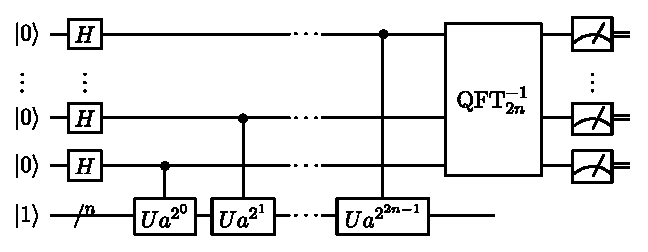
\includegraphics[width=12cm]{pic/Shor_algorithm.eps}
\caption{Circuit of Shor's algorithm}
\label{ShorAlgorithm}
\end{figure}

\subsection{Complexity}
